\section{Tries}
{\tiny a trie (or prefix tree) is a tree-based data structure, particularly used for fast
pattern matching \\
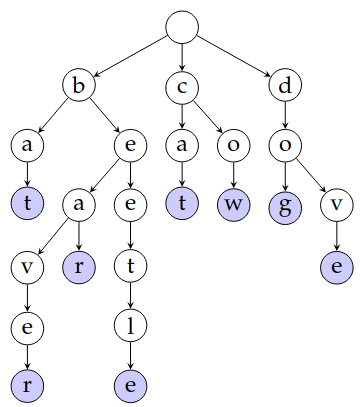
\includegraphics[scale=0.2]{trie.png}\\
}\\
\scriptsize{search}\\ 
{\tiny start from root, jump to node with current character\\
fail: if there is no character to follow/input ends in a non-leaf node\\
accpet if at a leaf node at the end of the input\\
to prevent that no string is a prefix of another: append a special end-of-string symbol/mark the nodes that correspond to ends of strings}\\
\scriptsize{complexity}\\
{\tiny O(n) for search, insert or delete\\
a factor from the alphabet size q, but can be reduced to O(log q) with binary search, or O(1) if a method allowing direct addressing is used
}\\
\scriptsize{properties}\\
{\tiny Internal nodes may have as many children as the number of symbols in the alphabet (in practice much smaller, averge degree of nodes goes down as the depth increase)\\
height of the trie=longest string\\
num of leaves = num of strings\\
worst case num of nodes=total length of all strings
}\\
\scriptsize{compress} {\tiny replace 'redundant' nodes with nodes labeled with substrings, saves space and may speed up operations
}\\
\scriptsize{suffix tries} {\tiny tries that include all suffixes of a string, O(n) for substring search\\
if the search ends in a leaf node, the pattern is a suffix of the string\\
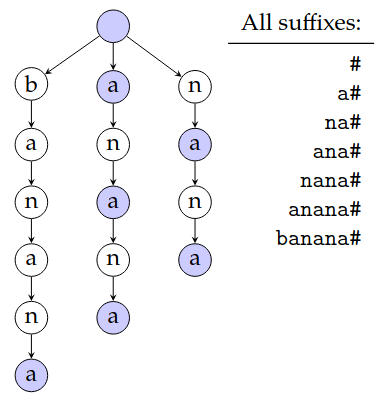
\includegraphics[scale=0.2]{suffix-trie.png}\\
Standard suffix tries use O(n**2) space, compression reduces space requirement to O(n), can be further reduced by keeping indexes to the string rather than the string itself in the (compressed) trie nodes\\
Iterative insertion of suffixes result in a quadratic (O(qn**2)) construction time complexity\\
there are linear time algorithms for constructing suffix tries\\
generalized suffix tries allow storing multiple strings(documents) in a single suffix trie (each string gets a special end-of-string marker)
}\\